\documentclass[hyperref={bookmarks=false},aspectratio=169]{beamer}
\usepackage{hyperref,ragged2e,amsmath,amssymb,url,bm}
\usepackage{graphicx,booktabs,array}
\usepackage{tikz}
\usetikzlibrary{arrows.meta,positioning,calc,shapes.geometric,decorations.pathreplacing,matrix}
\graphicspath{{crops/}}
\usetheme{Goettingen}
% --- Paleta de la serie Festividades santas: tierra roja, café rojizo, mostaza y papiro ---
\definecolor{tierraroja}{RGB}{122,40,18}
\definecolor{caferojizo}{RGB}{58,18,8}
\definecolor{mostaza}{RGB}{214,160,58}
\definecolor{papiro}{RGB}{243,228,192}
\definecolor{sepia}{RGB}{98,66,44}
\definecolor{oliva}{RGB}{92,98,48}
\setbeamercolor{structure}{fg=tierraroja}
\setbeamertemplate{sidebar canvas right}[vertical shading][top=tierraroja!92!black,bottom=caferojizo]
\setbeamercolor{title in sidebar}{fg=mostaza}
\setbeamercolor{author in sidebar}{fg=papiro}
\setbeamercolor{section in sidebar}{fg=papiro}
\setbeamercolor{section in sidebar shaded}{fg=mostaza!55!papiro!75!tierraroja}
\setbeamercolor{subsection in sidebar}{fg=papiro}
\setbeamercolor{subsection in sidebar shaded}{fg=mostaza!55!papiro!75!tierraroja}
\let\raggedright\justifying
\setlength{\RaggedRightRightskip}{0pt plus 1fil}
\setbeamertemplate{background canvas}{
\includegraphics[width=\paperwidth,height=\paperheight]{papiro.jpg}}
\setbeamercolor{normal text}{fg=caferojizo!90!black}
\setbeamercolor{frametitle}{fg=tierraroja}
\setbeamerfont{frametitle}{series=\bfseries}
\setbeamertemplate{section in toc shaded}{\leavevmode{\color{sepia!85!black}\inserttocsection}\par}
\setbeamercolor{title}{fg=tierraroja}
\setbeamercolor{subtitle}{fg=sepia}
\setbeamercolor{item projected}{bg=tierraroja,fg=papiro}
\setbeamertemplate{itemize item}{\small\textcolor{mostaza!80!tierraroja}{$\blacktriangleright$}}
\setbeamertemplate{navigation symbols}{}
% --- Español + hebreo + griego (XeLaTeX) con fuentes empaquetadas en fonts/ ---
\usepackage[bidi=default]{babel}
\babelprovide[import,main]{spanish}
\babelprovide[import]{hebrew}
\babelprovide[import]{ancientgreek}
\babelfont[hebrew]{sf}[Path=fonts/, BoldFont=NotoHebrewSans-700.ttf]{NotoHebrewSans-400.ttf}
\babelfont[hebrew]{rm}[Path=fonts/, BoldFont=NotoHebrewSans-700.ttf]{NotoHebrewSans-400.ttf}
\babelfont[ancientgreek]{sf}[Path=fonts/]{GFSPorson.otf}
\babelfont[ancientgreek]{rm}[Path=fonts/]{GFSPorson.otf}
\newcommand{\heb}[1]{\mbox{\foreignlanguage{hebrew}{#1}}}
\newcommand{\grc}[1]{\foreignlanguage{ancientgreek}{#1}}
\newcommand{\SENOR}{S{\fontsize{0.78em}{1em}\selectfont EÑOR}}
% --- Citas, imágenes, referencias ---
\usepackage[most]{tcolorbox}
\newtcolorbox{cita}[1][]{enhanced, colback=papiro, opacityback=0.80, colframe=tierraroja!85!mostaza,
  boxrule=0pt, leftrule=2.5pt, arc=0pt, left=6pt, right=6pt, top=4pt, bottom=4pt,
  before skip=4pt, after skip=6pt, fontupper=\small\itshape, #1}
\newcommand{\fuente}[1]{\par\hfill{\upshape\bfseries\footnotesize\textcolor{tierraroja}{#1}}}
\newcommand{\imagen}[3][0.80]{%
  \centering\includegraphics[height=#1\textheight,width=\linewidth,keepaspectratio]{#2}\par\vspace{2pt}
  {\fontsize{5}{6}\selectfont\color{sepia}{\raggedleft\textit{Nota.} #3\par}}}
\makeatletter
\newcommand{\fotolado}[2]{%
  \begin{tikzpicture}[remember picture,overlay]
    \node[anchor=north east,inner sep=0pt] (foto) at ([xshift=-\beamer@sidebarwidth]current page.north east)
      {\includegraphics[height=\paperheight]{#1}};
    \node[anchor=south east,inner sep=2pt,text=papiro,fill=caferojizo,fill opacity=0.55,text opacity=1,
      font=\fontsize{4.5}{5.5}\selectfont,align=right,text width=4.2cm] at ([xshift=-3pt,yshift=3pt]foto.south east)
      {\textit{Nota.} #2};
  \end{tikzpicture}}
\makeatother
\newcommand{\refapa}[1]{\par{\RaggedRight\hangindent=1.2em\hangafter=1\noindent #1\par}\vspace{3pt}}
\usepackage{xurl}\urlstyle{same}
\newcommand{\destacar}[1]{\textbf{\textcolor{tierraroja}{#1}}}
\newcommand{\precision}[1]{{\footnotesize\color{sepia}\textbf{Precisión:} #1}}
\newcolumntype{L}[1]{>{\RaggedRight\arraybackslash}p{#1}}
\tikzset{caja/.style={draw=tierraroja,line width=0.8pt,fill=papiro,fill opacity=0.90,text opacity=1,rounded corners=3pt,inner sep=5pt,font=\scriptsize}}
\title[El Jubileo]{\bfseries{El Jubileo: proclamaréis libertad en la tierra}}
\subtitle{``Pregonaréis libertad en la tierra a todos sus moradores'' (Lv 25:10)}
\author{}\institute{}\date{}
\titlegraphic{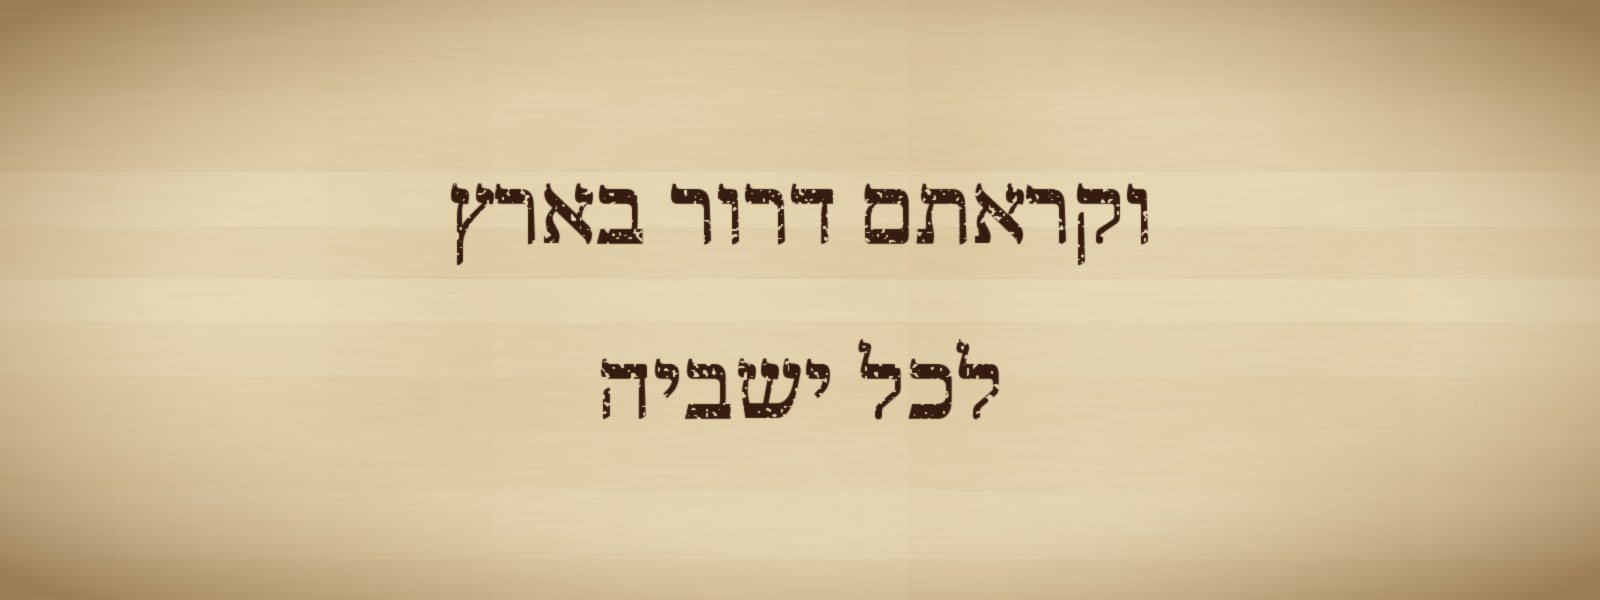
\includegraphics[width=0.80\linewidth,height=0.36\textheight,keepaspectratio]{portada.jpg}\\[-1pt]
  {\fontsize{5}{6}\selectfont\color{sepia}\textit{Nota.} Elaboración propia: Lv 25:10b en texto hebreo consonántico (BHS).}}
\begin{document}
\frame{\titlepage}


% ------------------------------------------------------------------
\section{Introducción}

\begin{frame}{La trompeta del día del perdón}
\begin{columns}[c,onlytextwidth]
\begin{column}{0.52\textwidth}
\begin{cita}Entonces harás tocar fuertemente la trompeta en el mes séptimo a los diez días del mes; el día de la expiación haréis tocar la trompeta por toda vuestra tierra.\fuente{(Lv 25:9)}\end{cita}
\small ¿Por qué la libertad se anuncia el \destacar{Día de la Expiación}, el día del ayuno y de la sangre en el Lugar Santísimo (Lv 16)?
\end{column}
\begin{column}{0.45\textwidth}
\begin{tcolorbox}[colback=papiro,colframe=tierraroja,boxrule=1pt,arc=3pt,left=4pt,right=4pt]
\small\textbf{Tesis.} El Jubileo lleva a la tierra, a la economía y a la familia lo que Yom Kipur realiza en el santuario: \destacar{Dios limpia primero y luego libera}.
\end{tcolorbox}
\scriptsize Fundamento: ``la tierra mía es'' (Lv 25:23) y ``son mis siervos, los cuales saqué yo de la tierra de Egipto'' (Lv 25:42).
\end{column}
\end{columns}
\end{frame}

\begin{frame}{El ciclo y el año cincuenta}
\centering
\resizebox{\linewidth}{!}{%
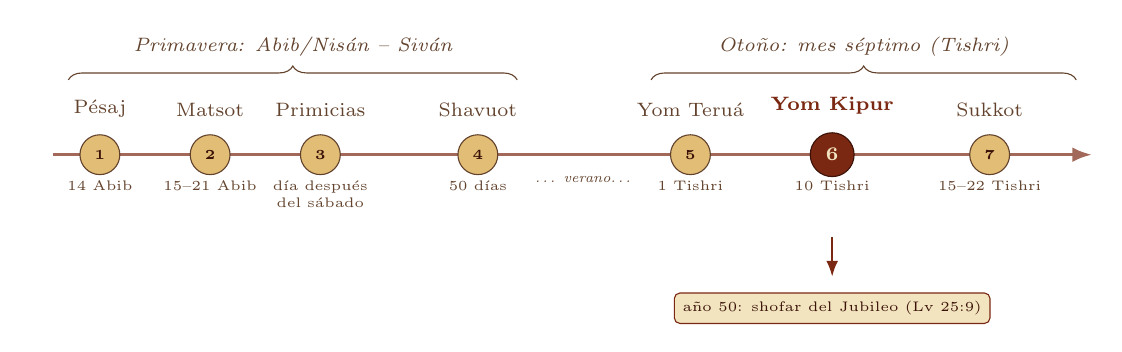
\begin{tikzpicture}[x=1cm,y=1cm,font=\scriptsize]
 \def\fiestaactual{6}
 \draw[line width=1.2pt,tierraroja!70,-{Latex[length=2.5mm]}] (0,0) -- (13.2,0);
 \draw[decorate,decoration={brace,amplitude=5pt},sepia] (0.2,0.95) -- (5.9,0.95) node[midway,above=5pt,font=\scriptsize\itshape]{Primavera: Abib/Nisán -- Siván};
 \draw[decorate,decoration={brace,amplitude=5pt},sepia] (7.6,0.95) -- (13.0,0.95) node[midway,above=5pt,font=\scriptsize\itshape]{Otoño: mes séptimo (Tishri)};
 \foreach \n/\x/\t/\d in {1/0.6/Pésaj/{14 Abib},2/2.0/Matsot/{15--21 Abib},3/3.4/Primicias/{día después del sábado},4/5.4/Shavuot/{50 días},5/8.1/Yom Teruá/{1 Tishri},6/9.9/Yom Kipur/{10 Tishri},7/11.9/Sukkot/{15--22 Tishri}}{
   \ifnum\n=\fiestaactual
     \node[circle,fill=tierraroja,draw=caferojizo,minimum size=5.5mm,text=papiro,font=\scriptsize\bfseries] at (\x,0) {\n};
     \node[above=3pt,font=\scriptsize\bfseries,text=tierraroja] at (\x,0.28) {\t};
   \else
     \node[circle,fill=mostaza!70,draw=sepia,minimum size=4.5mm,text=caferojizo,font=\tiny\bfseries] at (\x,0) {\n};
     \node[above=3pt,text=sepia] at (\x,0.25) {\t};
   \fi
   \node[below=6pt,text width=1.6cm,align=center,font=\tiny,text=sepia] at (\x,0) {\d};}
 \node[font=\tiny\itshape,text=sepia] at (6.75,-0.32) {\ldots\ verano\ldots};
 \draw[-{Latex[length=2mm]},tierraroja,line width=0.8pt] (9.9,-1.05) -- (9.9,-1.55);
 \node[draw=tierraroja,fill=papiro,rounded corners=2pt,font=\tiny,text=caferojizo,align=center,inner sep=3pt] at (9.9,-1.95) {año 50: shofar del Jubileo (Lv 25:9)};
\end{tikzpicture}}\par\medskip
\small\RaggedRight El Jubileo no figura entre las siete fiestas de Levítico 23, pues dura \destacar{un año} y no un día; con todo, se proclama dentro del ciclo, en la sexta solemnidad, el \destacar{10 de Tishri} del año cincuenta.
\end{frame}


% ------------------------------------------------------------------
\section{El texto}

\begin{frame}{Lv 25:8--10: la cuenta}
\fotolado{panel_levitico25.jpg}{Elaboración propia: Lv 25:10 en texto hebreo consonántico (BHS).}
\begin{columns}[c,onlytextwidth]
\begin{column}{0.57\textwidth}
\begin{cita}Y contarás siete semanas de años, siete veces siete años\ldots{} Entonces harás tocar fuertemente la trompeta en el mes séptimo a los diez días del mes\ldots{} Y santificaréis el año cincuenta, y pregonaréis libertad en la tierra a todos sus moradores; ese año os será de jubileo, y volveréis cada uno a vuestra posesión, y cada cual volverá a su familia.\fuente{(Lv 25:8--10)}\end{cita}
\scriptsize El pasaje encadena cuatro verbos: \destacar{contar}, hacer pasar el shofar, \destacar{santificar} y \destacar{proclamar}.
\end{column}
\begin{column}{0.41\textwidth}\end{column}
\end{columns}
\end{frame}

\begin{frame}{Lv 25:10 en hebreo}
\begin{center}
\heb{וּקְרָאתֶם דְּרוֹר בָּאָרֶץ לְכָל־יֹשְׁבֶיהָ יוֹבֵל הִוא תִּהְיֶה לָכֶם}\\[2pt]
\heb{וְשַׁבְתֶּם אִישׁ אֶל־אֲחֻזָּתוֹ וְאִישׁ אֶל־מִשְׁפַּחְתּוֹ תָּשֻׁבוּ}
\end{center}
\renewcommand{\arraystretch}{1.12}\scriptsize
\begin{tabular}{@{}L{2.9cm}L{1.2cm}L{7.6cm}@{}}
\toprule
\textbf{Término} & \textbf{Raíz} & \textbf{Sentido} \\ \midrule
\heb{וּקְרָאתֶם} \emph{ukratem} & \heb{קרא} & ``proclamaréis'': el verbo de \emph{mikrá kódesh}, ``convocación'' (``ensayo'', Strong H4744, es analogía) \\
\heb{דְּרוֹר} \emph{derór} & \heb{דרר} & ``liberación'': acto jurídico público; cognado del acadio \emph{andurārum} \\
\heb{יוֹבֵל} \emph{yovel} & \heb{יבל} & ``cuerno de carnero'': el año toma el nombre de su anuncio \\
\heb{אֲחֻזָּה} \emph{ajuzá} & \heb{אחז} & ``posesión'': lo que uno tiene asido; la tierra del clan \\
\heb{מִשְׁפָּחָה} \emph{mishpajá} & \heb{שׁפח} & ``familia, clan'': el grupo que sostiene el derecho de rescate \\
\bottomrule
\end{tabular}\par\smallskip
\small El versículo prevé dos retornos: \destacar{a la posesión} (la tierra) y \destacar{a la familia} (el clan).
\end{frame}

\begin{frame}{``La tierra mía es''}
\begin{center}\heb{וְהָאָרֶץ לֹא תִמָּכֵר לִצְמִתֻת כִּי־לִי הָאָרֶץ כִּי־גֵרִים וְתוֹשָׁבִים אַתֶּם עִמָּדִי}\end{center}
\begin{cita}La tierra no se venderá a perpetuidad, porque la tierra mía es; pues vosotros forasteros y extranjeros sois para conmigo.\fuente{(Lv 25:23)}\end{cita}
\begin{columns}[t,onlytextwidth]
\begin{column}{0.49\textwidth}\small
\begin{itemize}
\item \heb{לִצְמִתֻת} \emph{litsmitut}: venta que \destacar{extingue} el derecho (raíz ``acabar'').
\item Se venden \destacar{cosechas}, no la tierra (v.~15).
\end{itemize}
\end{column}
\begin{column}{0.49\textwidth}\small
\begin{itemize}
\item \emph{Guer ve-toshav}: residentes en tierra de Dios (Sal 39:12 [39:13]; 1~Cr 29:15).
\item LXX \grc{προσήλυτοι καὶ πάροικοι} → 1~P 2:11.
\end{itemize}
\end{column}
\end{columns}
\end{frame}

\begin{frame}{Tierra, casas y personas}
\centering
\begin{tikzpicture}[x=1cm,y=1cm,font=\scriptsize]
 \foreach \r/\c in {2.75/mostaza!25, 1.95/mostaza!40, 1.2/tierraroja!18}{\fill[\c] (0,0) circle (\r);}
 \foreach \r in {2.75,1.95,1.2}{\draw[tierraroja!70,line width=0.7pt] (0,0) circle (\r);}
 \fill[tierraroja] (0,0) circle (0.6);
 \node[text=papiro,font=\tiny\bfseries,align=center] at (0,0) {``Yo soy\\ el \SENOR''};
 \node[font=\scriptsize\bfseries,text=caferojizo] at (0,2.38) {Tierra {\tiny\mdseries vv.~13--28}};
 \node[font=\scriptsize\bfseries,text=caferojizo] at (0,1.6) {Casas {\tiny\mdseries 29--34}};
 \node[font=\scriptsize\bfseries,text=caferojizo] at (0,0.88) {Personas};
 \foreach \y/\t/\d in {2.0/{1. Vende tierra (v.~25)}/{rescata el \emph{goel} o él mismo; si no, vuelve en el Jubileo},
                       0.85/{2. Pide prestado (v.~35)}/{sin interés; vive contigo como residente},
                       -0.3/{3. Se vende a un israelita (v.~39)}/{jornalero, no esclavo; sale en el Jubileo},
                       -1.45/{4. Se vende a un extranjero (v.~47)}/{lo rescata un pariente; si no, sale en el Jubileo}}{
   \node[anchor=west,text width=6.2cm,align=left,font=\scriptsize] at (3.2,\y) {\textbf{\textcolor{tierraroja}{\t}}: \d};}
 \node[anchor=west,font=\tiny\itshape,text=sepia,text width=6.2cm] at (3.2,-2.45) {Cada caso se abre con \heb{כִּי־יָמוּךְ אָחִיךָ}, ``cuando tu hermano empobreciere''. Disposición en círculos: propuesta de lectura (cf. Milgrom, 2001).};
\end{tikzpicture}
\end{frame}

\begin{frame}{El precio según los años}
\centering
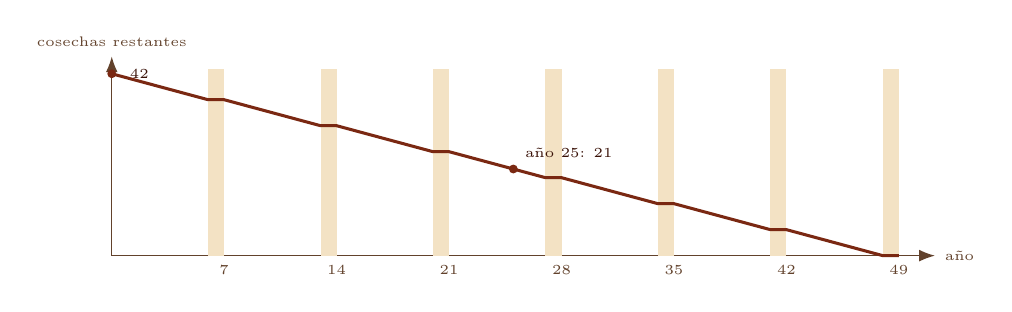
\begin{tikzpicture}[x=0.85cm,y=0.55cm,font=\scriptsize]
 \draw[sepia,line width=0.5pt,-{Latex[length=2mm]}] (0,0) -- (12.3,0) node[right,font=\tiny,text=sepia] {año};
 \draw[sepia,line width=0.5pt,-{Latex[length=2mm]}] (0,0) -- (0,4.6) node[above,font=\tiny,text=sepia] {cosechas restantes};
 \foreach \k in {7,14,21,28,35,42,49}{
   \fill[mostaza!30] ({(\k-1)*0.24},0) rectangle ({\k*0.24},4.3);
   \node[below,font=\tiny,text=sepia] at ({\k*0.24},0) {\k};}
 \draw[tierraroja,line width=1.1pt] plot coordinates {(0.00,4.20) (0.24,4.10) (0.48,4.00) (0.72,3.90) (0.96,3.80) (1.20,3.70) (1.44,3.60) (1.68,3.60) (1.92,3.50) (2.16,3.40) (2.40,3.30) (2.64,3.20) (2.88,3.10) (3.12,3.00) (3.36,3.00) (3.60,2.90) (3.84,2.80) (4.08,2.70) (4.32,2.60) (4.56,2.50) (4.80,2.40) (5.04,2.40) (5.28,2.30) (5.52,2.20) (5.76,2.10) (6.00,2.00) (6.24,1.90) (6.48,1.80) (6.72,1.80) (6.96,1.70) (7.20,1.60) (7.44,1.50) (7.68,1.40) (7.92,1.30) (8.16,1.20) (8.40,1.20) (8.64,1.10) (8.88,1.00) (9.12,0.90) (9.36,0.80) (9.60,0.70) (9.84,0.60) (10.08,0.60) (10.32,0.50) (10.56,0.40) (10.80,0.30) (11.04,0.20) (11.28,0.10) (11.52,0.00) (11.76,0.00)};
 \fill[tierraroja] (0,4.2) circle (1.6pt) node[right=3pt,font=\tiny,text=caferojizo] {42};
 \fill[tierraroja] (6.0,2.0) circle (1.6pt) node[above right=1pt,font=\tiny,text=caferojizo] {año 25: 21};
\end{tikzpicture}\par\smallskip
\begin{cita}Cuanto mayor fuere el número de los años, aumentarás el precio, y cuanto menor fuere el número, disminuirás el precio; porque según el número de las cosechas te venderá él.\fuente{(Lv 25:16)}\end{cita}
\vspace{-4pt}\justifying\precision{excluir los años sabáticos (bandas) del cómputo es lectura de comentaristas; el texto dice ``según el número de las cosechas''. ``No engañe ninguno a su prójimo, sino temed a vuestro Dios'' (v.~17).}
\end{frame}

\begin{frame}{Los textos legales}
\fontsize{6.6}{7.8}\selectfont\renewcommand{\arraystretch}{1.12}
\begin{tabular}{@{}L{1.9cm}L{2.5cm}L{7.6cm}@{}}
\toprule
\textbf{Texto} & \textbf{Tema} & \textbf{Qué añade} \\ \midrule
Éx 21:2--6 & Siervo hebreo & Sale libre el séptimo año; el que se queda sirve ``para siempre'' \\
Éx 23:10--11 & Año séptimo & La tierra descansa ``para que coman los pobres'' \\
Lv 25:1--7 & \emph{Shemitá} & ``la tierra tendrá descanso, reposo para \SENOR'' \\
Lv 25:8--12 & Cuenta y anuncio & 7\,×\,7 años; shofar el 10 del mes 7.º; \emph{derór}; posesión y familia \\
Lv 25:13--55 & Tierra, casas, personas & Precio por años; \emph{ge'ulá}; el \emph{goel}; préstamo sin interés; siervos \\
Lv 27:16--25 & Campos consagrados & En el Jubileo el campo vuelve a su dueño original (v.~24) \\
Nm 36:4 & Hijas de Zelofehad & El Jubileo no corrige una herencia pasada a otra tribu por matrimonio \\
Dt 15:1--18 & \emph{Shemitá} de deudas & Remisión de préstamos y liberación del siervo con provisiones \\
\bottomrule
\end{tabular}\par\smallskip
\par\justifying\precision{Éx 21 y Dt 15 liberan al siervo el séptimo año; Lv 25:40, ``hasta el año del jubileo''. Para la crítica, leyes de épocas distintas (Fager, 1993); para la tradición judía, el ``para siempre'' de Éx 21:6 es ``hasta el Jubileo'' (Rashi); otros ven en el Jubileo un tope absoluto (Wright, 2004).}
\end{frame}

\begin{frame}{Ecos en la narración y los profetas}
\fontsize{6.6}{7.8}\selectfont\renewcommand{\arraystretch}{1.12}
\begin{tabular}{@{}L{1.9cm}L{2.5cm}L{7.6cm}@{}}
\toprule
\textbf{Texto} & \textbf{Tema} & \textbf{Qué añade} \\ \midrule
Rut 2--4 & Booz, el \emph{goel} & Rescata el campo de Elimelec y se casa con Rut, en la puerta, ante los ancianos \\
1~R 21:3 & Nabot & ``Guárdeme \SENOR{} de que yo te dé a ti la heredad de mis padres'' \\
Jer 32:6--15 & Anatot & Jeremías redime el campo de su primo: ``Aún se comprarán casas, heredades y viñas'' \\
Jer 34:8--17 & Sedequías & \emph{Derór} pactado y revocado; Dios ``promulga libertad'' a la espada \\
Ez 46:16--18 & El príncipe & Lo dado a un siervo vuelve en \heb{שְׁנַת הַדְּרוֹר}, ``el año de la libertad'' (RVR1960: ``del jubileo'') \\
Neh 5; 10:31 & Crisis de deudas & Devolución de campos; promesa de guardar el año séptimo \\
Is 49:8--9; 58:6 & Siervo; ayuno & Restaurar la tierra, repartir heredades; ``dejar ir libres a los quebrantados'' \\
Is 61:1--3 & El ungido & \emph{Derór}, \emph{shenat ratsón} y ``el día de venganza'' \\
Lc 4:16--21 & Nazaret & ``Hoy se ha cumplido esta Escritura delante de vosotros'' \\
\bottomrule
\end{tabular}
\end{frame}

% ------------------------------------------------------------------
\section{Historia}

\begin{frame}{Tierra, clan y herencia}
\begin{columns}[c,onlytextwidth]
\begin{column}{0.50\textwidth}
\small\RaggedRight Tres niveles: tribu, clan (\emph{mishpajá}) y casa paterna (\emph{bet av}). La tierra se repartió \destacar{por suerte} (Nm 26:52--56; Jos 13--19): es \heb{נַחֲלָה} (\emph{najalá}), herencia, no mercancía.\par\medskip
\begin{cita}Guárdeme \SENOR{} de que yo te dé a ti la heredad de mis padres.\fuente{(1~R 21:3)}\end{cita}
\end{column}
\begin{column}{0.47\textwidth}
\begin{cita}¡Ay de los que juntan casa a casa, y añaden heredad a heredad hasta ocuparlo todo!\fuente{(Is 5:8)}\end{cita}
\scriptsize\RaggedRight Miqueas denuncia lo mismo: ``codician las heredades, y las roban'' (Mi 2:2). El hito narrado detrás del Jubileo es la \destacar{entrada en la tierra y el reparto}: ``Cuando hayáis entrado en la tierra que yo os doy'' (Lv 25:2).
\end{column}
\end{columns}
\end{frame}

\begin{frame}{Edictos de remisión}
\centering
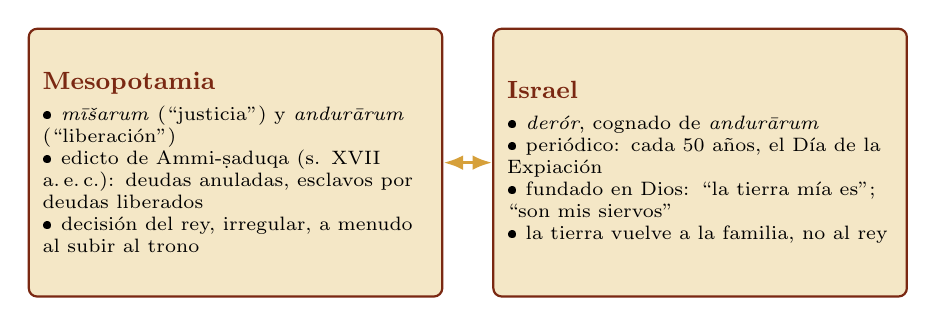
\begin{tikzpicture}[font=\scriptsize]
 \node[caja,text width=4.9cm,anchor=north,minimum height=3.4cm] (m) at (0,0) {{\small\textbf{\textcolor{tierraroja}{Mesopotamia}}}\\[3pt]\RaggedRight
   \textbullet\ \emph{mīšarum} (``justicia'') y \emph{andurārum} (``liberación'')\\
   \textbullet\ edicto de Ammi-ṣaduqa (s. XVII a.\,e.\,c.): deudas anuladas, esclavos por deudas liberados\\
   \textbullet\ decisión del rey, irregular, a menudo al subir al trono};
 \node[caja,text width=4.9cm,anchor=north,minimum height=3.4cm] (i) at (5.9,0) {{\small\textbf{\textcolor{tierraroja}{Israel}}}\\[3pt]\RaggedRight
   \textbullet\ \emph{derór}, cognado de \emph{andurārum}\\
   \textbullet\ periódico: cada 50 años, el Día de la Expiación\\
   \textbullet\ fundado en Dios: ``la tierra mía es''; ``son mis siervos''\\
   \textbullet\ la tierra vuelve a la familia, no al rey};
 \draw[{Latex[length=2.5mm]}-{Latex[length=2.5mm]},mostaza,line width=1.2pt] (m.east) -- (i.west);
\end{tikzpicture}\par\medskip
\scriptsize\RaggedRight Weinfeld (1995) mostró el trasfondo común (``proclamar \emph{derór}'' = fórmula real; ``juicio y justicia''); Lemche (1979), el carácter irregular de los edictos.\par
\par\justifying\precision{el paralelo ilumina la institución, aunque no la explica por completo: Israel la transforma.}
\end{frame}

\begin{frame}{¿Se practicó el Jubileo?}
\begin{columns}[t,onlytextwidth]
\begin{column}{0.48\textwidth}\scriptsize
\textbf{\textcolor{tierraroja}{Lo que dicen las fuentes}}
\begin{itemize}
\item Ningún relato narra un Jubileo.
\item Jer 34: \emph{derór} de Sedequías (ca. 588 a.\,e.\,c.), revocado; cita la ley del séptimo año.
\item Neh 5: remisión extraordinaria de deudas.
\item El año sabático sí está atestiguado (1~Mac 6:49, 53; Josefo).
\item Talmud: cesó con el exilio de Rubén, Gad y media Manasés, pues exige ``a todos sus moradores'' (b.~\emph{Arajin} 32b).
\end{itemize}
\end{column}
\begin{column}{0.50\textwidth}\scriptsize
\textbf{\textcolor{tierraroja}{Lo que discuten los autores}}
\begin{itemize}
\item \textbf{Ley ideal o tardía}: de Vaux (1985), utópica, nunca aplicada regularmente; Fager (1993), programa sacerdotal posexílico.
\item \textbf{Raíces antiguas}: Milgrom (2001), crisis agraria del s. VIII (Is 5:8; Mi 2:2); Bergsma (2007), sociedad tribal preexílica; Wright (2004), supone los clanes de Jos 13--19.
\end{itemize}
\par\justifying\precision{el silencio de las fuentes no prueba que la ley no existiera; indica, a lo sumo, que su cumplimiento fue difícil y que los profetas la recordaron como deuda pendiente.}
\end{column}
\end{columns}
\end{frame}

\begin{frame}{Jubileos y 11QMelquisedec}
\begin{columns}[t,onlytextwidth]
\begin{column}{0.48\textwidth}
\begin{tcolorbox}[colback=papiro,colframe=tierraroja,boxrule=0.8pt,arc=3pt,title={Libro de los Jubileos},fonttitle=\scriptsize\bfseries,coltitle=papiro,colbacktitle=tierraroja,left=3pt,right=3pt]
\scriptsize\RaggedRight Siglo II a.\,e.\,c. Toda la historia en \destacar{jubileos de 49 años} y ``semanas de años''. La entrada en Canaán llega al cumplirse \destacar{cincuenta jubileos} desde la creación (Jub 50:4). Calendario de 364 días (VanderKam, 1998, 2001).
\end{tcolorbox}
\end{column}
\begin{column}{0.50\textwidth}
\begin{tcolorbox}[colback=papiro,colframe=tierraroja,boxrule=0.8pt,arc=3pt,title={11QMelquisedec (11Q13)},fonttitle=\scriptsize\bfseries,coltitle=papiro,colbacktitle=tierraroja,left=3pt,right=3pt]
\scriptsize\RaggedRight Siglo I a.\,e.\,c. Une \destacar{Lv 25:13, Dt 15:2 e Is 61:1}: Melquisedec proclamará \emph{derór} a los cautivos para librarlos ``de la deuda de todas sus iniquidades''. El \destacar{Día de la Expiación} es el final del \destacar{décimo jubileo} (García Martínez, 1992; Vermes, 2004).
\end{tcolorbox}
\end{column}
\end{columns}
\medskip
\small\RaggedRight Un siglo antes de Jesús ya se leían juntos Levítico 25 e Isaías 61, ligados a la expiación, lo que enlaza este estudio con el de Yom Kipur.
\end{frame}

\begin{frame}{El Jubileo en la historia}
\centering
\resizebox{\linewidth}{!}{%
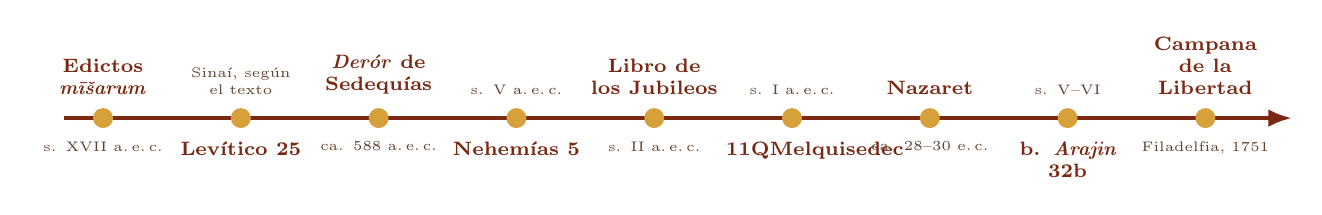
\begin{tikzpicture}[x=1cm,y=1cm,font=\scriptsize]
 \draw[line width=1.5pt,tierraroja,-{Latex[length=3mm]}] (0,0) -- (15.6,0);
 \foreach \x/\a/\b/\p in {0.5/{Edictos \emph{mīšarum}}/{s. XVII a.\,e.\,c.}/1, 2.25/{Levítico 25}/{Sinaí, según el texto}/0, 4.0/{\emph{Derór} de Sedequías}/{ca. 588 a.\,e.\,c.}/1, 5.75/{Nehemías 5}/{s. V a.\,e.\,c.}/0, 7.5/{Libro de los Jubileos}/{s. II a.\,e.\,c.}/1, 9.25/{11QMelquisedec}/{s. I a.\,e.\,c.}/0, 11.0/{Nazaret}/{ca. 28--30 e.\,c.}/1, 12.75/{b. \emph{Arajin} 32b}/{s. V--VI}/0, 14.5/{Campana de la Libertad}/{Filadelfia, 1751}/1}{
   \fill[mostaza] (\x,0) circle (3.6pt);
   \ifnum\p=1
     \node[above=5pt,text width=1.68cm,align=center,font=\scriptsize\bfseries,text=tierraroja] at (\x,0) {\a};
     \node[below=5pt,text width=1.68cm,align=center,font=\tiny,text=sepia] at (\x,0) {\b};
   \else
     \node[above=5pt,text width=1.68cm,align=center,font=\tiny,text=sepia] at (\x,0) {\b};
     \node[below=5pt,text width=1.68cm,align=center,font=\scriptsize\bfseries,text=tierraroja] at (\x,0) {\a};
   \fi}
\end{tikzpicture}}\par\medskip
{\scriptsize\RaggedRight
\textbf{1751.} Pensilvania encarga una campana para los 50 años de la Carta de 1701 con Lv 25:10: \emph{Proclaim liberty throughout all the land\ldots} (Nash, 2010).\par}\smallskip
\par\justifying\precision{uso posterior del término, no interpretación del texto.}
\end{frame}

% ------------------------------------------------------------------
\section{Filología}

\begin{frame}{\heb{יוֹבֵל} (\emph{yovel}): el cuerno}
\begin{columns}[t,onlytextwidth]
\begin{column}{0.54\textwidth}\scriptsize\renewcommand{\arraystretch}{1.15}
\begin{tabular}{@{}L{2.5cm}L{3.9cm}@{}}
\toprule
\textbf{Forma} & \textbf{Uso} \\ \midrule
\heb{שׁוֹפְרוֹת הַיּוֹבְלִים} & ``bocinas de cuernos de carnero'' en Jericó (Jos 6:4) \\
\heb{בְּקֶרֶן הַיּוֹבֵל} & ``el cuerno de carnero'' que suena largo (Jos 6:5) \\
\heb{בִּמְשֹׁךְ הַיֹּבֵל} & ``cuando suene largamente la bocina'' (Éx 19:13) \\
\heb{שְׁנַת הַיּוֹבֵל} & ``el año del jubileo'' (Lv 25:13) \\
\bottomrule
\end{tabular}
\end{column}
\begin{column}{0.44\textwidth}\small
\begin{itemize}
\item \destacar{27 veces} en el AT: 20 en Lv 25 y 27; 5 en Jos 6; Éx 19:13; Nm 36:4.
\item Sentido básico: \destacar{carnero}, y su cuerno (\emph{HALOT}); otros: \emph{yaval}, ``llevar''.
\item El latín \emph{iubilaeus} se cruzó con \emph{iubilare}: de ahí ``júbilo'', que no está en el hebreo.
\end{itemize}
\par\justifying\precision{conteo propio por lema sobre el Códice de Leningrado.}
\end{column}
\end{columns}
\end{frame}

\begin{frame}{\heb{דְּרוֹר} (\emph{derór}): liberación}
\begin{columns}[c,onlytextwidth]
\begin{column}{0.50\textwidth}\small
\begin{itemize}
\item \destacar{Siete veces} como ``liberación'': Lv 25:10; Is 61:1; Jer 34:8, 15, 17 (×2); Ez 46:17 (conteo propio).
\item Casi siempre con \emph{qará}, ``proclamar'': un \destacar{acto jurídico público}.
\item Cognado acadio: \emph{andurārum}.
\item Homónimos: \heb{דְּרוֹר} ``golondrina'' (Sal 84:3 [84:4]); \heb{מָר־דְּרוֹר} ``mirra que corre'' (Éx 30:23).
\end{itemize}
\end{column}
\begin{column}{0.47\textwidth}
\begin{cita}Vosotros no me habéis oído para promulgar cada uno libertad a su hermano\ldots{}; he aquí que yo promulgo libertad, dice \SENOR, a la espada y a la pestilencia y al hambre.\fuente{(Jer 34:17)}\end{cita}
\scriptsize El texto juega con el término: la libertad negada al hermano regresa como \destacar{libertad concedida al juicio}.
\end{column}
\end{columns}
\end{frame}

\begin{frame}{``Yo sé que mi Redentor vive''}
\fotolado{panel_job19.jpg}{Elaboración propia: Job 19:25 en texto hebreo consonántico (BHS).}
\begin{columns}[c,onlytextwidth]
\begin{column}{0.57\textwidth}
\begin{cita}Yo sé que mi Redentor vive, Y al fin se levantará sobre el polvo.\fuente{(Job 19:25)}\end{cita}
\scriptsize\RaggedRight
\heb{גָּאַל} \emph{ga'al}: rescatar lo que es de la familia: campo (Lv 25:25), casa (v.~29), persona (vv.~48--49).\\[2pt]
\heb{גֹּאֵל} \emph{goel}: el pariente con derecho y deber de rescatar (Rut 3:9, 12); \emph{goel hadam}, vengador de la sangre (Nm 35:19).\\[2pt]
Dios es \emph{goel}: ``os redimiré'' (Éx 6:6); ``tu Redentor, el Santo de Israel'' (Is 41:14); ``\SENOR{} Rey de Israel, y su Redentor'' (Is 44:6).\\[2pt]
\emph{Padá}: rescate por pago; \emph{ga'al}: rescate \destacar{por parentesco}.
\end{column}
\begin{column}{0.41\textwidth}\end{column}
\end{columns}
\end{frame}

\begin{frame}{Posesión, heredad, forasteros}
\scriptsize\renewcommand{\arraystretch}{1.15}
\begin{tabular}{@{}L{2.7cm}L{9.2cm}@{}}
\toprule
\textbf{Término} & \textbf{Sentido y usos} \\ \midrule
\heb{אֲחֻזָּה} \emph{ajuzá} & ``Posesión'', lo que uno tiene asido (\emph{ajaz}); clave de Lv 25; ``heredad perpetua'' prometida a Abraham (Gn 17:8) \\
\heb{נַחֲלָה} \emph{najalá} & ``Heredad'' asignada por suerte (Nm 26:52--56); Israel es la heredad de Dios (Dt 32:9) \\
\heb{לִצְמִתֻת} \emph{litsmitut} & ``A perpetuidad'': solo Lv 25:23, 30; LXX \grc{εἰς βεβαίωσιν} \\
\heb{גֵּר} \emph{guer} & ``Forastero'': Abraham en Hebrón (Gn 23:4) \\
\heb{תּוֹשָׁב} \emph{toshav} & ``Residente''; LXX \grc{πάροικος}; ``extranjeros y peregrinos'' (1~P 2:11) \\
\heb{שְׁנַת רָצוֹן} \emph{shenat ratsón} & ``Año de la buena voluntad'' (Is 61:2); \emph{ratsón} es la ofrenda ``aceptada'' (Lv 1:3); LXX \grc{δεκτός} \\
\bottomrule
\end{tabular}\par\medskip
\small El israelita no es dueño absoluto, sino \destacar{residente en la tierra de Dios}; en esa condición, la Iglesia, ``extranjera y peregrina'' (He 11:13), espera una heredad.
\end{frame}

\begin{frame}{De \emph{derór} a \emph{áphesis}}
\centering
\resizebox{\linewidth}{!}{%
\begin{tikzpicture}[font=\small,node distance=0.55cm]
 \node[caja,font=\small,text width=3.0cm,align=center] (h) {\textbf{Hebreo}\\[2pt] \heb{דְּרוֹר} \emph{derór}\\ {\scriptsize Lv 25:10; Is 61:1}};
 \node[caja,font=\small,text width=3.0cm,align=center,right=of h] (l) {\textbf{Septuaginta}\\[2pt] \grc{ἄφεσις}\\ {\scriptsize \grc{ἐνιαυτὸς ἀφέσεως}; Is 58:6}};
 \node[draw=mostaza,line width=1.4pt,fill=tierraroja,text=papiro,rounded corners=3pt,text width=3.0cm,align=center,inner sep=5pt,right=of l] (n) {\textbf{Lucas 4:18}\\[2pt] \grc{ἄφεσιν}\ +\ \grc{ἐν ἀφέσει}\\ {\scriptsize dos ``liberaciones''}};
 \node[caja,font=\small,text width=3.0cm,align=center,right=of n] (e) {\textbf{NT}\\[2pt] \grc{ἄφεσις ἁμαρτιῶν}\\ {\scriptsize Lc 24:47; Ef 1:7}};
 \draw[-{Latex[length=3mm]},mostaza,line width=1.3pt] (h)--(l);
 \draw[-{Latex[length=3mm]},mostaza,line width=1.3pt] (l)--(n);
 \draw[-{Latex[length=3mm]},mostaza,line width=1.3pt] (n)--(e);
\end{tikzpicture}}\par\smallskip
{\footnotesize\itshape\color{sepia} La liberación del Jubileo y el perdón de los pecados se expresan con una misma palabra griega.}\par\medskip
\scriptsize\RaggedRight\textbf{El rescate en griego:} \grc{λυτρόω} traduce \emph{ga'al} (Lv 25:25); \grc{ἀγχιστεύς}, el \emph{goel} de Rut; \grc{λύτρον} (Mc 10:45); \grc{ἐξαγοράζω} (Gá 3:13; 4:5); \grc{ἀπολύτρωσις}, ``la redención de la posesión adquirida'' (Ef 1:14) y ``de nuestro cuerpo'' (Ro 8:23); \grc{ἀποκατάστασις}, ``restauración de todas las cosas'' (Hch 3:21).
\end{frame}

% ------------------------------------------------------------------
\section{Texto}

\begin{frame}{Lucas 4:18: ``libertad''}
\fotolado{panel_lucas4.jpg}{Elaboración propia: Lc 4:18b en escritura uncial (texto NA28).}
\begin{columns}[c,onlytextwidth]
\begin{column}{0.57\textwidth}
\begin{cita}El Espíritu del Señor está sobre mí, Por cuanto me ha ungido para dar buenas nuevas a los pobres; Me ha enviado a sanar a los quebrantados de corazón; A pregonar libertad a los cautivos, Y vista a los ciegos; A poner en libertad a los oprimidos; A predicar el año agradable del Señor.\fuente{(Lc 4:18--19)}\end{cita}
\scriptsize \grc{κηρύξαι αἰχμαλώτοις ἄφεσιν\ldots{} ἀποστεῖλαι τεθραυσμένους ἐν ἀφέσει}: la palabra del Jubileo, \destacar{dos veces}.
\end{column}
\begin{column}{0.41\textwidth}\end{column}
\end{columns}
\end{frame}

\begin{frame}{Is 61 frente a Lc 4}
\fontsize{6.4}{7.6}\selectfont\renewcommand{\arraystretch}{1.12}
\begin{tabular}{@{}L{3.9cm}L{3.9cm}L{4.1cm}@{}}
\toprule
\textbf{Is 61:1--2 (TM, RVR1960)} & \textbf{LXX} & \textbf{Lc 4:18--19} \\ \midrule
me ungió \SENOR; buenas nuevas a los abatidos & \grc{εὐαγγελίσασθαι πτωχοῖς} & dar buenas nuevas a los pobres \\
vendar a los quebrantados de corazón & \grc{ἰάσασθαι τοὺς συντετριμμένους} & sanar a los quebrantados (\emph{falta en NA28}) \\
publicar libertad (\emph{derór}) a los cautivos & \grc{κηρύξαι αἰχμαλώτοις ἄφεσιν} & pregonar libertad a los cautivos \\
a los presos apertura de la cárcel & \grc{καὶ τυφλοῖς ἀνάβλεψιν} & y vista a los ciegos \\
--- & (Is 58:6) \grc{ἐν ἀφέσει} & poner en libertad a los oprimidos \\
el año de la buena voluntad de \SENOR & \grc{ἐνιαυτὸν κυρίου δεκτόν} & el año agradable del Señor \\
\destacar{y el día de venganza del Dios nuestro} & \grc{καὶ ἡμέραν ἀνταποδόσεως} & \destacar{(no lo lee: ``enrollando el libro\ldots{} se sentó'')} \\
\bottomrule
\end{tabular}\par\medskip
\small\RaggedRight Jesús \destacar{interrumpe la lectura a mitad de versículo} y declara: ``Hoy se ha cumplido esta Escritura delante de vosotros'' (Lc 4:21).
\end{frame}

\begin{frame}{Precisión textual y significado}
\begin{columns}[t,onlytextwidth]
\begin{column}{0.49\textwidth}\scriptsize\RaggedRight
\textbf{\textcolor{tierraroja}{1. Is 58:6 insertado.}} Unión de textos por una palabra común (\emph{gezerá shavá}); ¿composición lucana o lectura sinagogal? (Fitzmyer, 1981; Nolland, 1989; Bock, 1994).\par\medskip
\textbf{\textcolor{tierraroja}{2. ``Sanar a los quebrantados''.}} En el Texto Mayoritario y el \emph{Textus Receptus} (RVR1960); falta en \heb{א}, B, D, L, W: armonización con Is 61:1 LXX.
\end{column}
\begin{column}{0.49\textwidth}\scriptsize\RaggedRight
\textbf{\textcolor{tierraroja}{3. ``Vista a los ciegos''.}} \heb{פְּקַח־קוֹחַ} (\emph{peqaj-qóaj}): forma rara; \emph{paqaj} es ``abrir los ojos'' (Is 42:7), y la LXX leyó ``vista''.\par\medskip
\textbf{\textcolor{tierraroja}{4. La frase omitida.}} Para muchos, distinción entre la gracia presente y el juicio futuro (Bock, 1994); el juicio no se anula: ``días de retribución'' (Lc 21:22).\par\medskip
\textbf{\textcolor{tierraroja}{5. Ap 5:9.}} ``Nos has redimido'' (\grc{ἡμᾶς}): falta en A; NA28 \grc{ἠγόρασας τῷ θεῷ}.
\end{column}
\end{columns}
\end{frame}

\begin{frame}{¿Año 49 o 50?}
\begin{columns}[t,onlytextwidth]
\begin{column}{0.52\textwidth}\scriptsize
\begin{itemize}
\item \textbf{Año 50 aparte}: dos años seguidos sin siembra (49 y 50); opinión de los sabios (b.~\emph{Nedarim} 61a).
\item \textbf{Cómputo inclusivo}: el 50 es el 1 del ciclo siguiente, como el día 50 de Shavuot; R. Yehudá: ``cuenta para ambos lados''; ciclos de 49 en Jubileos (Bergsma, 2007).
\item \textbf{Año de otoño a otoño}: el anuncio del 10 de Tishri; Hoenig (1969) propuso un período intercalar breve.
\end{itemize}
\end{column}
\begin{column}{0.46\textwidth}
\begin{tcolorbox}[colback=papiro,colframe=mostaza!85!tierraroja,boxrule=0.8pt,arc=2pt,left=3pt,right=3pt,title={Del 1 al 10 de Tishri},fonttitle=\scriptsize\bfseries,coltitle=caferojizo,colbacktitle=mostaza!35]
\scriptsize\RaggedRight Según el Talmud, los siervos no volvían a casa ni servían: comían y bebían ``con sus coronas en la cabeza''; en Yom Kipur sonaba el shofar y salían (b.~\emph{Rosh Hashaná} 8b).
\end{tcolorbox}
\par\justifying\precision{Dn 9:24 (``setenta semanas'' = 490 años = diez jubileos) y la cuenta de ``120 jubileos'' desde Adán (material de Yom Kipur de la serie) son lecturas cronológicas, no datos del texto.}
\end{column}
\end{columns}
\end{frame}

% ------------------------------------------------------------------
\section{Literatura}

\begin{frame}{Siete por siete más uno}
\centering
\resizebox{\linewidth}{!}{%
\begin{tikzpicture}[x=1cm,y=1cm,font=\scriptsize]
 \node[anchor=east,font=\scriptsize\bfseries,text=caferojizo,align=right] at (-0.2,1.3) {Shavuot\\ {\tiny\mdseries Lv 23:15--16}};
 \node[anchor=east,font=\scriptsize\bfseries,text=caferojizo,align=right] at (-0.2,0) {Jubileo\\ {\tiny\mdseries Lv 25:8--10}};
 \foreach \i in {1,...,7}{
   \node[draw=sepia,fill=mostaza!25,minimum width=1.25cm,minimum height=0.7cm,font=\tiny,align=center] at ({(\i-1)*1.4+0.65},1.3) {semana \i\\ 7 días};
   \node[draw=sepia,fill=mostaza!25,minimum width=1.25cm,minimum height=0.7cm,font=\tiny,align=center] at ({(\i-1)*1.4+0.65},0) {\emph{shemitá} \i\\ 7 años};}
 \node[draw=tierraroja,fill=tierraroja,text=papiro,minimum width=1.9cm,minimum height=0.8cm,font=\tiny\bfseries,align=center] (s) at (11.0,1.3) {día 50\\ Shavuot};
 \node[draw=tierraroja,fill=tierraroja,text=papiro,minimum width=1.9cm,minimum height=0.8cm,font=\tiny\bfseries,align=center] (j) at (11.0,0) {año 50\\ \emph{yovel}};
 \draw[-{Latex[length=2mm]},tierraroja,line width=0.8pt] (9.55,1.3) -- (s.west);
 \draw[-{Latex[length=2mm]},tierraroja,line width=0.8pt] (9.55,0) -- (j.west);
 \draw[decorate,decoration={brace,amplitude=5pt},sepia] (0,1.85) -- (9.4,1.85) node[midway,above=5pt,font=\tiny,text=sepia] {\heb{וּסְפַרְתֶּם} ``contaréis'': 7 × 7 = 49 días};
 \draw[decorate,decoration={brace,amplitude=5pt,mirror},sepia] (0,-0.55) -- (9.4,-0.55) node[midway,below=5pt,font=\tiny,text=sepia] {\heb{וְסָפַרְתָּ} ``contarás'': 7 × 7 = 49 años};
\end{tikzpicture}}\par\medskip
\small\RaggedRight Ambas cuentas usan el mismo verbo (\emph{safar}) y la misma fórmula (\heb{שֶׁבַע שַׁבָּתוֹת}). El 50 funciona como un \destacar{octavo}, a la vez sábado de los sábados y \destacar{primer año de un ciclo nuevo}, a semejanza del octavo día de Sukkot (Lv 23:36).
\end{frame}

\begin{frame}{El ciclo de cuarenta y nueve}
\centering
\begin{tikzpicture}[x=0.5cm,y=0.5cm,font=\tiny]
 \foreach \c in {1,...,7}{\node[text=sepia] at (\c,0.45) {\c};}
 \foreach \r in {1,...,7}{
  \node[anchor=east,text=sepia] at (0.35,{-\r+0.5}) {ciclo \r};
  \foreach \c in {1,...,7}{
   \pgfmathtruncatemacro{\y}{(\r-1)*7+\c}
   \ifnum\c=7
     \fill[tierraroja!75] (\c-0.5,-\r) rectangle (\c+0.5,-\r+1);
     \node[text=papiro,font=\tiny\bfseries] at (\c,{-\r+0.5}) {\y};
   \else
     \fill[mostaza!25] (\c-0.5,-\r) rectangle (\c+0.5,-\r+1);
     \node[text=caferojizo] at (\c,{-\r+0.5}) {\y};
   \fi
   \draw[sepia!70,line width=0.3pt] (\c-0.5,-\r) rectangle (\c+0.5,-\r+1);}}
 \node[draw=tierraroja,line width=1pt,fill=tierraroja,text=papiro,minimum width=1.9cm,minimum height=1.9cm,font=\small\bfseries,align=center] (cin) at (11.2,-3.5) {50\\[1pt] {\scriptsize\mdseries \heb{יוֹבֵל}}};
 \draw[-{Latex[length=2.5mm]},tierraroja,line width=1pt] (7.6,-6.5) to[out=0,in=-90] (cin.south);
 \node[anchor=west,text width=4.2cm,font=\scriptsize,align=left] at (14,-2.3) {\textbf{\textcolor{tierraroja}{7, 14\ldots{} 49:}} \emph{shemitá}, sábado de la tierra (Lv 25:1--7).};
 \node[anchor=west,text width=4.2cm,font=\scriptsize,align=left] at (14,-4.7) {\textbf{\textcolor{tierraroja}{50:}} shofar el 10 de Tishri, Día de la Expiación; \emph{derór}, posesión, familia.};
\end{tikzpicture}\par\medskip
\scriptsize Pocos verían más de un Jubileo, de modo que el período equivale a \destacar{una generación}.
\end{frame}

\begin{frame}{La estructura de Levítico 25}
\begin{columns}[c,onlytextwidth]
\begin{column}{0.55\textwidth}\small
\begin{itemize}
\item Marco: ``en el monte de Sinaí'' (25:1; 26:46; 27:34).
\item \destacar{``Cuando tu hermano empobreciere''} (vv.~25, 35, 39, 47): espiral descendente de la pobreza.
\item \destacar{``Temed a vuestro Dios''} (vv.~17, 36, 43): la sanción es el temor de Dios.
\item \destacar{``Que os saqué de la tierra de Egipto''} (vv.~38, 42, 55): el éxodo como razón última.
\end{itemize}
\scriptsize\RaggedRight\textbf{Síntesis de la serie:} 1. sabático (1--7); 2. Jubileo (8--17); 2.1 obediencia (18--22); 2.2 santidad de la tierra: rescate (23--34) y del pueblo: préstamo y manumisión (35--55); cierre: ``Guardad mis días de reposo (26:2).
\end{column}
\begin{column}{0.42\textwidth}
\begin{tcolorbox}[colback=papiro,colframe=tierraroja,boxrule=0.8pt,arc=3pt,left=4pt,right=4pt]
\centering\small\textbf{\textcolor{tierraroja}{La tríada de Lv 25:10}}\\[4pt]
\scriptsize \emph{derór} → libertad\\ \emph{ajuzá} → posesión\\ \emph{mishpajá} → familia\\[4pt]
\RaggedRight Se trata de \destacar{restitución} y no de caridad: el tiempo devuelve cada cosa al reparto original.
\end{tcolorbox}
\end{column}
\end{columns}
\end{frame}

\begin{frame}{Isaías 61: el heraldo}
\fotolado{panel_isaias61.jpg}{Elaboración propia: Is 61:1 en texto hebreo consonántico (BHS).}
\begin{columns}[c,onlytextwidth]
\begin{column}{0.57\textwidth}
\begin{cita}El Espíritu de \SENOR{} el Señor está sobre mí, porque me ungió \SENOR; me ha enviado a predicar buenas nuevas a los abatidos, a vendar a los quebrantados de corazón, a publicar libertad a los cautivos, y a los presos apertura de la cárcel; a proclamar el año de la buena voluntad de \SENOR, y el día de venganza del Dios nuestro\ldots\fuente{(Is 61:1--2)}\end{cita}
\scriptsize\RaggedRight El ungido ejerce el oficio del \destacar{heraldo del Jubileo}. Is 49:8--9 añade: restaurar la tierra, heredar heredades, ``decir a los presos: Salid''; Pablo: ``he aquí ahora el día de salvación'' (2~Co 6:2).
\end{column}
\begin{column}{0.41\textwidth}\end{column}
\end{columns}
\end{frame}



% ------------------------------------------------------------------
\section{El goel}

\begin{frame}{Las cuatro funciones del \emph{goel}}
\begin{columns}[c,onlytextwidth]
\begin{column}{0.56\textwidth}
\centering
\begin{tikzpicture}[font=\scriptsize]
 \node[draw=tierraroja,line width=1pt,fill=tierraroja,text=papiro,rounded corners=3pt,align=center,inner sep=4pt,font=\small\bfseries] (cen) at (0,0) {\emph{goel}\\[1pt] {\heb{גֹּאֵל}}};
 \foreach \a/\n/\t/\r in {135/1/{Recuperar la tierra}/{Lv 25:25}, 45/2/{Rescatar a la persona}/{Lv 25:47--49}, -45/3/{Vengar la sangre}/{Nm 35:12--34}, -135/4/{Preservar el nombre}/{Dt 25:5--10; Rut 3--4}}{
   \node[caja,text width=2.45cm,align=center] (f\n) at (\a:2.25cm) {\textbf{\textcolor{tierraroja}{\n. \t}}\\ {\tiny\color{sepia}(\r)}};
   \draw[-{Latex[length=2mm]},mostaza,line width=1pt] (cen) -- (f\n);}
\end{tikzpicture}
\end{column}
\begin{column}{0.42\textwidth}\scriptsize\RaggedRight
\emph{Goel}: participio activo de \heb{גאל}, ``recuperar, redimir''. En cada caso la \destacar{casa paterna está en peligro} y el pariente preserva ``las condiciones mínimas de su existencia'' (Winters, 1994, p.~25).\par\medskip
Orden fijo: hermano, tío, primo, pariente (Lv 25:48--49): ``hay pariente más cercano que yo'' (Rut 3:12).\par\medskip
Raíz \emph{g'l}: 118 veces (verbo 104 + \emph{gueulá} 14); Lv 31, Isaías 24 (17 en caps. 40--55), Rut 23 (López, 1994).\par\smallskip
\precision{cifras de López confirmadas por conteo propio por lema (Códice de Leningrado), salvo Is 40--55. La función 4 es el levirato (Dt 25), que Rut combina con el \emph{goel}; Job 19:25 (no 9:25).}
\end{column}
\end{columns}
\end{frame}

\begin{frame}{Rut 4: el rescate en la puerta}
\centering
\resizebox{\linewidth}{!}{%
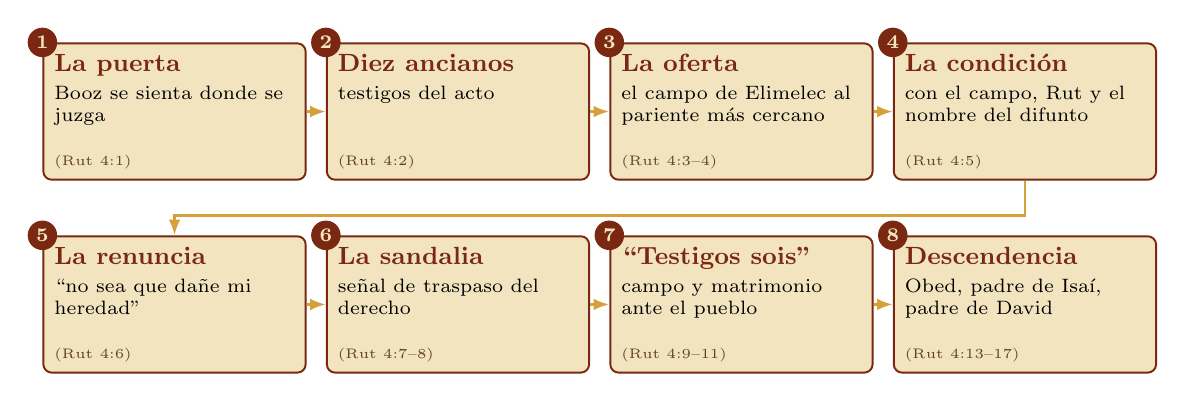
\begin{tikzpicture}[font=\scriptsize]
 \foreach \x/\y/\n/\t/\d/\r in {0/0/1/{La puerta}/{Booz se sienta donde se juzga}/{4:1},
                                 3.6/0/2/{Diez ancianos}/{testigos del acto}/{4:2},
                                 7.2/0/3/{La oferta}/{el campo de Elimelec al pariente más cercano}/{4:3--4},
                                 10.8/0/4/{La condición}/{con el campo, Rut y el nombre del difunto}/{4:5},
                                 0/-2.45/5/{La renuncia}/{``no sea que dañe mi heredad''}/{4:6},
                                 3.6/-2.45/6/{La sandalia}/{señal de traspaso del derecho}/{4:7--8},
                                 7.2/-2.45/7/{``Testigos sois''}/{campo y matrimonio ante el pueblo}/{4:9--11},
                                 10.8/-2.45/8/{Descendencia}/{Obed, padre de Isaí, padre de David}/{4:13--17}}{
  \node[draw=tierraroja,line width=0.7pt,fill=papiro,rounded corners=3pt,anchor=north,inner sep=4pt] (b\n) at (\x,\y) {\parbox[t][1.45cm][t]{3.05cm}{\RaggedRight{\small\textbf{\textcolor{tierraroja}{\t}}}\\[2pt]\scriptsize \d\par\vfill{\tiny\color{sepia}(Rut \r)}}};
  \node[circle,fill=tierraroja,text=papiro,font=\scriptsize\bfseries,inner sep=1.5pt] at (b\n.north west) {\n};}
 \foreach \a/\b in {1/2,2/3,3/4,5/6,6/7,7/8}{\draw[-{Latex[length=2mm]},mostaza,line width=1pt] (b\a.east) -- (b\b.west);}
 \draw[-{Latex[length=2mm]},mostaza,line width=1pt] (b4.south) -- (b4.south |- 0,-2.2) -| (b5.north);
\end{tikzpicture}}\par\medskip
\small\RaggedRight ``Extiende el borde de tu capa sobre tu sierva, \destacar{por cuanto eres pariente cercano}'' (Rut 3:9; \heb{כִּי גֹאֵל אָתָּה}). El niño es ``restaurador de tu alma'' (Rut 4:15).\par
\par\justifying\precision{Rut combina el rescate de Lv 25:25 con una obligación cercana al levirato (Dt 25:5--10); la relación es discutida (Hubbard, 1988).}
\end{frame}

\begin{frame}{Jeremías compra en la ruina}
\begin{columns}[c,onlytextwidth]
\begin{column}{0.52\textwidth}
\begin{cita}Porque así ha dicho \SENOR{} de los ejércitos, Dios de Israel: Aún se comprarán casas, heredades y viñas en esta tierra.\fuente{(Jer 32:15)}\end{cita}
\end{column}
\begin{column}{0.45\textwidth}\small\RaggedRight
Babilonia sitia Jerusalén. Hanameel ofrece a su primo el campo de Anatot, porque a él \destacar{le corresponde el rescate}. Jeremías paga, firma ante testigos y guarda la escritura en una vasija de barro (Jer 32:9--14).\par\medskip
Jeremías convierte así la ley del \emph{goel} en \destacar{promesa de retorno}.
\end{column}
\end{columns}
\end{frame}

\begin{frame}{El Redentor en Isaías}
\begin{columns}[t,onlytextwidth]
\begin{column}{0.53\textwidth}\scriptsize\renewcommand{\arraystretch}{1.12}
\begin{tabular}{@{}L{2.1cm}L{4.1cm}@{}}
\toprule
\textbf{Título} & \textbf{Texto} \\ \midrule
Santo de Israel & ``tu Redentor, el Santo de Israel'' (41:14) \\
Creador y Rey & ``Creador de Israel, vuestro Rey'' (43:14--15) \\
\SENOR{} de los ejércitos & ``Rey de Israel, y su Redentor'' (44:6) \\
Fuerte de Jacob & ``Redentor tuyo, el Fuerte de Jacob'' (49:26) \\
Esposo; Padre & ``tu marido es tu Hacedor'' (54:5); ``nuestro Redentor perpetuo'' (63:16) \\
\bottomrule
\end{tabular}
\end{column}
\begin{column}{0.45\textwidth}
\begin{cita}No temas, porque yo te redimí; te puse nombre, mío eres tú.\fuente{(Is 43:1)}\end{cita}
\scriptsize\RaggedRight Dos rescates: el \destacar{éxodo} (Is 51:10; 63:9) y \destacar{Babilonia} (48:20; 52:3, ``sin dinero seréis rescatados''). El pueblo se llamará ``Redimidos de \SENOR'' (62:12; cf. 35:9--10). En Is 41--63, ``Redentor'' 13 veces, todas el participio \emph{goel} (conteo propio). Arango (1994): un Dios \destacar{solidario} con su pueblo.
\end{column}
\end{columns}
\end{frame}

\begin{frame}{``El año de mis redimidos''}
\begin{columns}[c,onlytextwidth]
\begin{column}{0.48\textwidth}
\centering\heb{כִּי יוֹם נָקָם בְּלִבִּי וּשְׁנַת גְּאוּלַי בָּאָה}
\begin{cita}Porque el día de la venganza está en mi corazón, y el año de mis redimidos ha llegado.\fuente{(Is 63:4)}\end{cita}
\begin{cita}\ldots{}y la casa de Jacob recuperará sus posesiones.\fuente{(Abd 17)}\end{cita}
\end{column}
\begin{column}{0.50\textwidth}
\centering
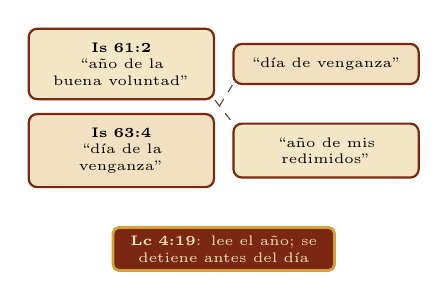
\begin{tikzpicture}[font=\tiny]
 \node[caja,text width=2.0cm,align=center,font=\tiny] (a1) at (0,1.1) {\textbf{Is 61:2}\\ ``año de la buena voluntad''};
 \node[caja,text width=2.0cm,align=center,font=\tiny,fill=mostaza!35] (a2) at (2.6,1.1) {``día de venganza''};
 \node[caja,text width=2.0cm,align=center,font=\tiny,fill=mostaza!35] (b1) at (0,0) {\textbf{Is 63:4}\\ ``día de la venganza''};
 \node[caja,text width=2.0cm,align=center,font=\tiny] (b2) at (2.6,0) {``año de mis redimidos''};
 \draw[sepia,dashed] (a1.south east) -- (b2.north west);
 \draw[sepia,dashed] (a2.south west) -- (b1.north east);
 \node[draw=mostaza,line width=1pt,fill=tierraroja,text=papiro,rounded corners=2pt,text width=2.6cm,align=center,inner sep=3pt] (l) at (1.3,-1.25) {\textbf{Lc 4:19}: lee el año; se detiene antes del día};
\end{tikzpicture}\par\smallskip
\scriptsize\RaggedRight Is 63 y Abdías apuntan contra \destacar{Edom}: tras el día del \SENOR{} (Abd 15), la casa de Jacob \destacar{recupera sus posesiones} y ``el reino será de \SENOR'' (Abd 21). Eco en Ap 19:13--15 (``pisa el lagar'').\par
\precision{Is 63:4 dice \emph{ge'ulay}, no \emph{yovel}: leerlo como Jubileo final (así la serie: ``el año de mi redención (Jubileo) ha llegado'') es tipológico.}
\end{column}
\end{columns}
\end{frame}

% ------------------------------------------------------------------
\section{La serie}

\begin{frame}{Memorial, figura y esperanza}
\begin{columns}[c,onlytextwidth]
\begin{column}{0.50\textwidth}\scriptsize\RaggedRight
La serie lee Lv 23 como el \destacar{Reglamento del Culto}: cada fiesta es memorial de un hito de Israel y figura del plan de salvación. El Jubileo no es convocación de Lv 23, pero el texto lo une al marco:
\begin{enumerate}
\item \textbf{Convocación}: se anuncia ``el día de la expiación'' (Lv 25:9).
\item \textbf{Hito}: la entrada en la tierra y el reparto (Lv 25:2; Jos 13--21).
\item \textbf{Esperanza}: Is 61; ``redención de la posesión adquirida'' (Ef 1:14); ``restauración de todas las cosas'' (Hch 3:21).
\end{enumerate}
\end{column}
\begin{column}{0.47\textwidth}
\begin{cita}El año del Jubileo era el Día de Expiación\ldots{} El verdadero cumplimiento del año del Jubileo tomará lugar en la segunda venida del Mesías.\fuente{(Yom Kipur, material de la serie)}\end{cita}
\scriptsize Expiación → \destacar{libertad} → \destacar{retorno a la heredad}.
\end{column}
\end{columns}
\end{frame}

\begin{frame}{La secuencia del otoño}
\centering
\resizebox{\linewidth}{!}{%
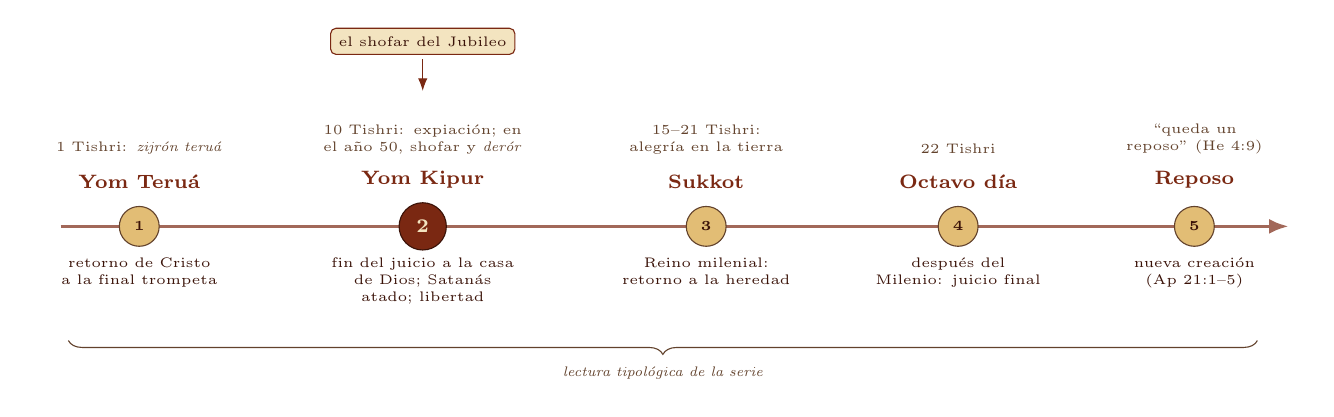
\begin{tikzpicture}[x=1cm,y=1cm,font=\scriptsize]
 \draw[line width=1.3pt,tierraroja!70,-{Latex[length=2.5mm]}] (0,0) -- (15.6,0);
 \foreach \x/\n/\t/\d/\s in {1.0/1/{Yom Teruá}/{1 Tishri: \emph{zijrón teruá}}/{retorno de Cristo a la final trompeta},
                             4.6/2/{Yom Kipur}/{10 Tishri: expiación; en el año 50, shofar y \emph{derór}}/{fin del juicio a la casa de Dios; Satanás atado; libertad},
                             8.2/3/{Sukkot}/{15--21 Tishri: alegría en la tierra}/{Reino milenial: retorno a la heredad},
                             11.4/4/{Octavo día}/{22 Tishri}/{después del Milenio: juicio final},
                             14.4/5/{Reposo}/{``queda un reposo'' (He 4:9)}/{nueva creación (Ap 21:1--5)}}{
   \ifnum\n=2
    \node[circle,fill=tierraroja,draw=caferojizo,minimum size=6mm,text=papiro,font=\scriptsize\bfseries] at (\x,0) {\n};
   \else
    \node[circle,fill=mostaza!70,draw=sepia,minimum size=5mm,text=caferojizo,font=\tiny\bfseries] at (\x,0) {\n};
   \fi
   \node[above=6pt,font=\scriptsize\bfseries,text=tierraroja] at (\x,0.15) {\t};
   \node[above=17pt,font=\tiny,text=sepia,text width=2.6cm,align=center] at (\x,0.2) {\d};
   \node[below=8pt,font=\tiny,text=caferojizo,text width=2.6cm,align=center] at (\x,0) {\s};}
 \draw[decorate,decoration={brace,amplitude=5pt,mirror},sepia] (0.1,-1.45) -- (15.2,-1.45) node[midway,below=6pt,font=\tiny\itshape,text=sepia] {lectura tipológica de la serie};
 \node[draw=tierraroja,fill=papiro,rounded corners=2pt,font=\tiny,align=center,inner sep=3pt,text=caferojizo] at (4.6,2.35) {el shofar del Jubileo};
 \draw[-{Latex[length=1.6mm]},tierraroja] (4.6,2.12) -- (4.6,1.72);
\end{tikzpicture}}\par\medskip
\scriptsize\RaggedRight El shofar recorre toda la secuencia: memorial (Lv 23:24), liberación (Lv 25:9), ``final trompeta'' (1~Co 15:52). ``Se tocará con gran trompeta, y vendrán los que habían sido esparcidos'' (Is 27:13).\par
\par\justifying\precision{el vínculo del Jubileo con la segunda venida, el Milenio o la nueva creación es lectura tipológica; el texto establece el anuncio en Yom Kipur (Lv 25:9) y Lc 4 lo aplica a Jesús. En Jericó sonaron ``las bocinas de \emph{yovel}'' (Jos 6:4).}
\end{frame}

% ------------------------------------------------------------------
\section{Mesías}

\begin{frame}{``Hoy se ha cumplido''}
\begin{columns}[c,onlytextwidth]
\begin{column}{0.50\textwidth}
\begin{cita}Y enrollando el libro, lo dio al ministro, y se sentó; y los ojos de todos en la sinagoga estaban fijos en él. Y comenzó a decirles: Hoy se ha cumplido esta Escritura delante de vosotros.\fuente{(Lc 4:20--21)}\end{cita}
\end{column}
\begin{column}{0.47\textwidth}\scriptsize
\begin{itemize}
\item \destacar{El heraldo}: el ungido pregona \grc{ἄφεσις} como Israel proclamaba \emph{derór}.
\item \destacar{El tiempo}: ``el año agradable'' designa un año, y ``hoy'' (\grc{σήμερον}) lo declara presente.
\item \destacar{El alcance}: la viuda de Sarepta y Naamán el sirio (Lc 4:25--27).
\item \destacar{Las obras}: ``a los pobres es anunciado el evangelio'' (Lc 7:22; Mt 11:5).
\end{itemize}
\end{column}
\end{columns}
\end{frame}

\begin{frame}{Cristo, el \emph{goel}}
\centering
\resizebox{\linewidth}{!}{%
\begin{tikzpicture}[font=\scriptsize,node distance=0.55cm]
 \node[caja,text width=3.0cm,align=center] (a) {\textbf{El pariente}\\[2pt] rescata campo y persona\\ {\tiny (Lv 25:25, 48--49; Rut 4)}};
 \node[caja,text width=3.0cm,align=center,right=of a] (b) {\textbf{Dios, \emph{goel} de Israel}\\[2pt] del éxodo al retorno\\ {\tiny (Éx 6:6; Is 41:14; 44:6)}};
 \node[caja,text width=3.0cm,align=center,right=of b] (c) {\textbf{``Mi Redentor vive''}\\[2pt] \heb{גֹּאֲלִי חָי}\\ {\tiny (Job 19:25)}};
 \node[draw=mostaza,line width=1.4pt,fill=tierraroja,text=papiro,rounded corners=3pt,text width=3.0cm,align=center,inner sep=5pt,right=of c] (d) {\textbf{Cristo, el hermano}\\[2pt] ``nacido de mujer''\\ {\tiny (Gá 4:4--5; He 2:14--15; Ap 5:9)}};
 \draw[-{Latex[length=3mm]},mostaza,line width=1.3pt] (a)--(b);
 \draw[-{Latex[length=3mm]},mostaza,line width=1.3pt] (b)--(c);
 \draw[-{Latex[length=3mm]},mostaza,line width=1.3pt] (c)--(d);
\end{tikzpicture}}\par\medskip
\begin{cita}\ldots{}Dios envió a su Hijo, nacido de mujer y nacido bajo la ley, para que redimiese a los que estaban bajo la ley, a fin de que recibiésemos la adopción de hijos.\fuente{(Gá 4:4--5)}\end{cita}
\justifying\scriptsize El derecho de rescate pertenece al pariente, y por ello \destacar{el Redentor se hace hermano} (He 2:11, 14). ``Con tu sangre nos has redimido para Dios'' (Ap 5:9).\par
\par\justifying\precision{autoría de Hebreos discutida (Lane, 1991); Gá 4:4--5, carta indiscutida, dice lo mismo.}
\end{frame}

\begin{frame}{La creación liberada}
\begin{columns}[t,onlytextwidth]
\begin{column}{0.49\textwidth}
\begin{cita}Porque también la creación misma será libertada de la esclavitud de corrupción, a la libertad gloriosa de los hijos de Dios.\fuente{(Ro 8:21)}\end{cita}
\scriptsize Primicias (Shavuot), adopción (retorno a la familia), \destacar{redención del cuerpo} (Ro 8:23): la \emph{ge'ulá} del Jubileo.
\end{column}
\begin{column}{0.49\textwidth}
\begin{cita}\ldots{}hasta los tiempos de la restauración de todas las cosas, de que habló Dios por boca de sus santos profetas.\fuente{(Hch 3:21)}\end{cita}
\scriptsize Pecados borrados → tiempos de refrigerio → \grc{ἀποκατάστασις} (Hch 3:19--21). Cristo libra ``a todos los que por el temor de la muerte estaban durante toda la vida sujetos a servidumbre'' (He 2:15).
\end{column}
\end{columns}
\end{frame}


% ------------------------------------------------------------------
\section{Tradición}

\begin{frame}{El Jubileo en la tradición judía}
\begin{columns}[t,onlytextwidth]
\begin{column}{0.49\textwidth}\scriptsize
\begin{itemize}
\item El shofar del Jubileo se equipara al de Rosh Hashaná (m.~\emph{Rosh Hashaná} 3:5).
\item Los siervos salían en Yom Kipur (b.~\emph{Rosh Hashaná} 8b).
\item Suspendido desde el exilio de las tribus (b.~\emph{Arajin} 32b; \emph{Sifra}, \emph{Behar}); Maimónides, \emph{Hiljot Shemitá ve-Yovel}.
\item Hillel instituye el \emph{prozbul} para preservar las deudas ante la \emph{shemitá} (m.~\emph{Sheviit} 10:3--4).
\end{itemize}
\par\justifying\precision{fuentes de los siglos II--XII e.\,c.; describen la interpretación rabínica, no necesariamente la práctica bíblica.}
\end{column}
\begin{column}{0.49\textwidth}\scriptsize
\textbf{\textcolor{tierraroja}{Debate: ¿Lucas 4 social o espiritual?}}
\begin{itemize}
\item \textbf{Social}: Yoder (1972), un Jubileo real; Ringe (1985), imágenes de liberación en Lucas; Sloan (1977), teología jubilar.
\item \textbf{Escatológico y espiritual}: Lucas no nombra el Jubileo; la \grc{ἄφεσις} es perdón (Fitzmyer, 1981; Bock, 1994).
\item \textbf{Integral}: paradigma ético, tipo cumplido en Cristo y esperanza escatológica (Wright, 2004).
\end{itemize}
\end{column}
\end{columns}
\end{frame}

% ------------------------------------------------------------------
\section{Síntesis}

\begin{frame}{Definición}
\begin{tcolorbox}[colback=papiro,colframe=tierraroja,boxrule=1pt,arc=3pt,left=5pt,right=5pt,title={El Jubileo},fonttitle=\small\bfseries,coltitle=papiro,colbacktitle=tierraroja]
\small\RaggedRight El \destacar{año cincuenta}, después de siete ciclos sabáticos, anunciado con el shofar el \destacar{10 de Tishri, Día de la Expiación} (Lv 25:8--9). Se proclama \emph{derór}: cada uno vuelve a su posesión y a su familia, la tierra descansa y el hermano vendido sale libre (Lv 25:10--13, 39--41). Su fundamento: la tierra y el pueblo son de Dios (Lv 25:23, 42). Los profetas lo hicieron imagen de la restauración (Is 61); Jesús lo declaró cumplido ``hoy'' (Lc 4:21); Cristo es el pariente que rescata (Gá 4:4--5). En la lectura de la serie: \destacar{expiación, libertad y retorno a la heredad}, hasta el reposo que queda (He 4:9).
\end{tcolorbox}
\begin{columns}[t,onlytextwidth]
\begin{column}{0.49\textwidth}
\begin{cita}Por tanto, queda un reposo para el pueblo de Dios.\fuente{(He 4:9)}\end{cita}
\end{column}
\begin{column}{0.49\textwidth}
\begin{cita}He aquí, yo hago nuevas todas las cosas.\fuente{(Ap 21:5)}\end{cita}
\end{column}
\end{columns}
\end{frame}

\begin{frame}{Lectura y aporte}
\fontsize{6.6}{7.8}\selectfont\renewcommand{\arraystretch}{1.18}
\begin{tabular}{@{}L{2.0cm}L{10.0cm}@{}}
\toprule
\textbf{Lectura} & \textbf{Aporte} \\ \midrule
Histórica & Protege el reparto por clanes; transforma la remisión mesopotámica (\emph{andurārum}) en ley periódica, divina y familiar; relectura escatológica en Jubileos y 11QMelquisedec \\
Filológica & \emph{Yovel}, el cuerno; \emph{derór}, la liberación; \emph{goel}, el pariente; LXX \grc{ἄφεσις}, la palabra del perdón \\
Textual & Lc 4 une Is 61:1--2 LXX con Is 58:6 y se detiene antes del ``día de venganza''; el año rige desde Yom Kipur \\
Literaria & 7\,×\,7\,+\,1 como Shavuot; círculos de redención (tierra, casas, personas); Rut 4 y Jer 32 narran al \emph{goel} \\
Serie & Nace de la Expiación: perdón, libertad, heredad; figura del Reino y del reposo final (tipología) \\
Nuevo Testamento & Cristo heraldo ungido y pariente redentor; \grc{ἀπολύτρωσις} del cuerpo y de la creación; \grc{ἀποκατάστασις} \\
\bottomrule
\end{tabular}
\end{frame}

% ------------------------------------------------------------------
\section{Reflexión}

\begin{frame}{Para la reflexión}
\small
\begin{enumerate}
\item ``Vosotros forasteros y extranjeros sois para conmigo'' (Lv 25:23): ¿qué cambia al tener, comprar o vender si uno es residente y no dueño absoluto?
\item ``Temed a vuestro Dios'' es la única sanción del precio justo y del préstamo sin interés (vv.~17, 36): ¿en qué casos ese temor es la única garantía del otro?
\item Booz aceptó el costo que el otro pariente rechazó (Rut 4:6): ¿qué enseña sobre el precio de la redención (1~P 1:18--19)?
\item Jeremías compró un campo en la ruina (Jer 32): ¿qué gestos de esperanza son posibles hoy?
\item ``Hoy'' (Lc 4:21), ``ahora'' (2~Co 6:2): ¿cómo vivir en el año agradable mientras se espera la redención del cuerpo (Ro 8:23)?
\item Nazaret se enojó cuando la liberación alcanzó a extranjeros (Lc 4:25--29): ¿a quién dejaríamos fuera del Jubileo?
\end{enumerate}
\end{frame}

% ------------------------------------------------------------------
\section{Glosario}

\begin{frame}{Glosario}
\fontsize{6.4}{7.6}\selectfont
\begin{columns}[t,onlytextwidth]
\begin{column}{0.49\textwidth}
\begin{description}\setlength{\itemsep}{1pt}
\item[\emph{Ajuzá}] (\heb{אֲחֻזָּה}) posesión asida; clave de Lv 25.
\item[\emph{Andurārum}] (acadio) liberación de deudas y esclavos; cognado de \emph{derór}.
\item[\emph{Áphesis}] (\grc{ἄφεσις}) remisión; Jubileo en la LXX; perdón en el NT.
\item[\emph{Apokatástasis}] (\grc{ἀποκατάστασις}) restauración (Hch 3:21).
\item[\emph{Apolytrōsis}] (\grc{ἀπολύτρωσις}) redención completa (Ro 8:23; Ef 1:14).
\item[\emph{Dektós}] (\grc{δεκτός}) aceptable: ``año agradable'' (Lc 4:19).
\item[\emph{Derór}] (\heb{דְּרוֹר}) liberación proclamada (Lv 25:10; Is 61:1).
\item[\emph{Ge'ulá}] (\heb{גְּאֻלָּה}) rescate: derecho y precio (Lv 25:24).
\end{description}
\end{column}
\begin{column}{0.49\textwidth}
\begin{description}\setlength{\itemsep}{1pt}
\item[\emph{Goel}] (\heb{גֹּאֵל}) pariente redentor; título de Dios (Is 44:6; Job 19:25).
\item[\emph{Guer ve-toshav}] (\heb{גֵּר וְתוֹשָׁב}) forastero y residente (Lv 25:23).
\item[\emph{Mīšarum}] (acadio) edicto real de ``justicia'' y remisión.
\item[\emph{Najalá}] (\heb{נַחֲלָה}) heredad asignada por suerte (1~R 21:3).
\item[\emph{Shemitá}] (\heb{שְׁמִטָּה}) año séptimo; remisión de deudas (Dt 15:1--2).
\item[\emph{Shenat ratsón}] (\heb{שְׁנַת רָצוֹן}) año de la buena voluntad (Is 61:2).
\item[\emph{Tsemitut}] (\heb{צְמִתֻת}) perpetuidad: venta definitiva (Lv 25:23, 30).
\item[\emph{Yovel}] (\heb{יוֹבֵל}) cuerno de carnero; el año cincuenta.
\end{description}
\end{column}
\end{columns}
\end{frame}

% ------------------------------------------------------------------
\section{Referencias}

\begin{frame}{Referencias}
\fontsize{4.6}{5.5}\selectfont
\begin{columns}[t,onlytextwidth]
\begin{column}{0.49\textwidth}
\refapa{Bergsma, J.~S. (2007). \emph{The Jubilee from Leviticus to Qumran: A history of interpretation}. Brill.}
\refapa{Bock, D.~L. (1994). \emph{Luke 1:1--9:50} (BECNT). Baker.}
\refapa{De Vaux, R. (1985). \emph{Instituciones del Antiguo Testamento}. Herder.}
\refapa{Elliger, K., \& Rudolph, W. (Eds.). (1997). \emph{Biblia Hebraica Stuttgartensia} (5.ª ed.). Deutsche Bibelgesellschaft.}
\refapa{Fager, J.~A. (1993). \emph{Land tenure and the biblical Jubilee}. JSOT Press.}
\refapa{Fitzmyer, J.~A. (1981). \emph{The Gospel according to Luke I--IX} (AB 28). Doubleday.}
\refapa{García Martínez, F. (1992). \emph{Textos de Qumrán}. Trotta.}
\refapa{Hartley, J.~E. (1992). \emph{Leviticus} (WBC 4). Word Books.}
\refapa{Hoenig, S.~B. (1969). Sabbatical years and the year of Jubilee. \emph{The Jewish Quarterly Review, 59}(3), 222--236.}
\refapa{Hubbard, R.~L. (1988). \emph{The book of Ruth} (NICOT). Eerdmans.}
\refapa{Koehler, L., \& Baumgartner, W. (2001). \emph{The Hebrew and Aramaic lexicon of the Old Testament}. Brill.}
\refapa{Lane, W.~L. (1991). \emph{Hebrews 1--8} (WBC 47A). Word Books.}
\refapa{Lemche, N.~P. (1979). Andurārum and mīšarum. \emph{Journal of Near Eastern Studies, 38}(1), 11--22.}
\refapa{Milgrom, J. (2001). \emph{Leviticus 23--27} (AB 3B). Doubleday.}
\refapa{Nash, G.~B. (2010). \emph{The Liberty Bell}. Yale University Press.}
\end{column}
\begin{column}{0.49\textwidth}
\refapa{Nestle, E., \& Aland, K. (Eds.). (2012). \emph{Novum Testamentum Graece} (28.ª ed.). Deutsche Bibelgesellschaft.}
\refapa{Nolland, J. (1989). \emph{Luke 1--9:20} (WBC 35A). Word Books.}
\refapa{Rahlfs, A., \& Hanhart, R. (Eds.). (2006). \emph{Septuaginta} (ed. rev.). Deutsche Bibelgesellschaft.}
\refapa{Ringe, S.~H. (1985). \emph{Jesus, liberation, and the biblical Jubilee}. Fortress Press.}
\refapa{\emph{Santa Biblia: Reina-Valera 1960}. (1960). Sociedades Bíblicas en América Latina.}
\refapa{Sloan, R.~B. (1977). \emph{The favorable year of the Lord}. Schola Press.}
\refapa{Steinsaltz, A. (Ed.). (2017). \emph{Koren Talmud Bavli} [RH 8b; Arajin 12a, 32b; Nedarim 61a]. Sefaria.}
\refapa{VanderKam, J.~C. (1998). \emph{Calendars in the Dead Sea Scrolls}. Routledge.}
\refapa{VanderKam, J.~C. (2001). \emph{The Book of Jubilees}. Sheffield Academic Press.}
\refapa{Vermes, G. (2004). \emph{The complete Dead Sea Scrolls in English} (ed. rev.). Penguin.}
\refapa{Weinfeld, M. (1995). \emph{Social justice in ancient Israel and in the ancient Near East}. Fortress Press.}
\refapa{Wenham, G.~J. (1979). \emph{The book of Leviticus} (NICOT). Eerdmans.}
\refapa{Wright, C.~J.~H. (2004). \emph{Old Testament ethics for the people of God}. InterVarsity Press.}
\refapa{Yoder, J.~H. (1972). \emph{The politics of Jesus}. Eerdmans.}
\par\smallskip{\color{sepia}Citas bíblicas: RVR1960; ``Jehová'' se reemplaza por \SENOR. Hebreo: BHS; griego: NA28 y LXX. Lo rabínico y las lecturas tipológicas se marcan como \emph{precisión}.}
\end{column}
\end{columns}
\end{frame}

\end{document}
